\chapter{ Introduction} 
\label{chap1}
%%%%%%%%%%%%%%%%%%%%%%%%%%%%%%%%%%%%%%%%

%\section{Overview}
In this chapter, we will give a basic overview of the problem that we are trying to solve and why we chose to solve this problem. We will start off by explaining the purpose of the project and the document. Then we will talk about what AR is and, how it is different from VR, how it is impacting the way users interact with the technology and how it is making it easier to access information without cluttering the workspace of the user. Then we will move on to how it could be used in Location Tracking systems to give a better understanding of the whereabouts of the user. At the end, we will give a brief introduction of the technologies that we will use in the implementation of our proposed system.

%%%%%%%%%%%%%%%%%%%%%%%%%%%%%%%%%%%%%%%%%%%%%%%%%%%%%%%%%%%%%%%%%

\section{Purpose of the Project}
Man is a social animal. We have a strong desire to connect with others, share our experiences with one another. We care deeply for our loved ones and want to keep track of them, to know where they are at a particular time. Parents want to keep track of their children, and friends want to find one another in crowds easily. It makes us feel more secure and closer to each other.

Augmented Reality (AR) is a type of technology that superimposes virtual objects onto the real world. Although there are a number of apps already out there that provide the feature of user tracking, none of them is using Augmented Reality to give a better user experience. By using AR in a location tracking app, the user will be able to better visualize where and how far someone is at the current moment. Imagine that you are in a crowded space and you quickly want to find your friend in the crowd. With AR supported app, you would open up the app, and it would point out the location of your friend in the crowd by showing a marker at his location, in the real-world.

Our proposed system will be using GPS (Global Positioning System), along with other technologies like WiFi, Cellular network etc, to get the current location of the user and update it in the remote real-time database. Once a user's location is updated, it will be reflected to all the contacts of the user so they could easily see where that user is at the current moment. The system will use AR (augmented reality) along with Google Maps, for the visualization of a user's location. 

\section{Purpose of this Document}
This document serves to be a report describing and explaining the process and the procedures taken to develop a tracking system that manages a user's contacts and their locations in real-time and, along with Google Maps, uses augmented reality for the visualization of their location at a particular time.

\section{Overview of this Document}
This report is divided into 5 chapters:
\begin{itemize}
	  \item Chapter \ref{chap1} introduces the main idea of the project, the purpose of the project/document. It also briefly describes the technologies that are used in the proposed system.
    \item Chapter \ref{chap2} describes the devised design of the software system, its architecture, different modules involved; data flow throughout the system, data schema for the database, and some design and implementation constraints.
    \item Chapter \ref{chap3} gives the implementation details of the software system and the problem that we encountered during the development.
    \item Chapter \ref{chap4} evaluates the achievements of this project and if it achieved its objectives.
    \item Chapter \ref{chap5} gives the conclusion of the project as well as some guidelines to further develop and improve the project in future.
		%\item Chapter \ref{chap6} shows some future directions that the project might take and how it could be improved further.
    %\item Chapter \ref{chap8} reflects on what we learned throughout this project.
\end{itemize}


\section{Objectives} \label{objectives}
The core objectives of the project are:
\begin{itemize}
    \item Design and implement a system that tracks a user location and stores it in a remote database in real-time.
    \item Implement some social features so that a user can add other users into his contact list and keep track of their location at all times.
    \item Add real-time chatting functionality in the application for easier communication between users when navigating.
    \item Use Augmented Reality for the visualization of the user marker in the real-world at any specific interval.
    \item Add in-app chat-bot that provides guidance and assistance to the user in using the app effectively.
    \item The devised system should be economical, for the end-user as well as for the developers.
\end{itemize}

%\section{Achievements}
%This project claims the following achievements:
%\begin{enumerate}
    %\item Designed and implemented a system that authenticates a user and then tracks his location and updates it in a real-time remote database as soon as it changes.
    %\item Other users can be added to the contact list of the currently logged in user. Location details of the contacts are fetched from the remote database in real-time and are displayed as markers on a map.
    %\item User can send chat messages to his contacts in real-time.
    %\item Augmented Reality is used, where it is supported, to show the location markers of the contacts in real-world.
    %\item Chat-bot is integrated into the app that provides helpful feedback and guidance to the user, to make his experience more effective and enjoyable.
    %\item The technologies used to design and implement this system are completely free. 
%\end{enumerate}

\section{Augmented Reality}
Augmented Reality (AR) is a type of technology that is used to overlay virtual graphical content onto the real world \cite{silva2003introduction}. It is a variation of Virtual Reality (VR) but instead of replacing the real world completely, as, in VR, it augments or supplements the real-world by superimposing virtual content onto the real world. In an ideal scenario, the user will not be able to tell the difference between the virtual and real objects in the same space. Figure \ref{fig:ar-example-ikea} shows an example of such a scene where a virtual sofa and a lamp is superimposed on a real-world space, augmenting the experience of the user to show him what it would feel like if there really was a sofa like that present there.

\begin{figure}
    \centering
        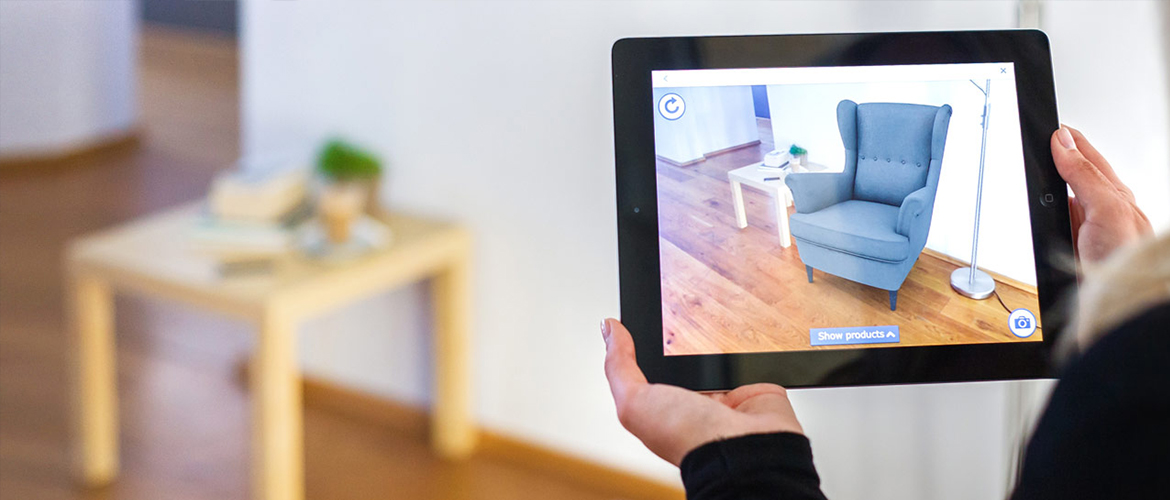
\includegraphics[width=1.00\textwidth]{images/ar-example-ikea.jpg}
    \caption{AR example with virtual sofa}
    \label{fig:ar-example-ikea}
\end{figure}

\subsection{Motivation}
We chose to use Augmented Reality in our application because of its utility and effectiveness in conveying the information, which is not readily available to a user in a real-world scenario, without secluding him from the reality.

Although Virtual Reality technology has its own benefits, for example, in providing an immersive experience which could be used for educational, tourism, simulation purposes, etc., the main drawback of VR is that it completely secludes the user from real-world. In contrast, the AR technology does not remove the user from the real world, but it augments the real-world around the user in order to provide him with extra information that he could not detect with his senses. This dramatically increases the utility of the AR technology as it could be used for numerous applications without affecting the work-flow of the user \cite{schmalstieg2016augmented}. 

\subsection{Applications}
Every interaction technology has its own benefits and applications. Although touch screens are quite easy and effective to use, they are not suitable for usage in every environment. Similarly, text-based interfaces are pretty outdated, but still, there are still some cases where they turn out to be the best way to interact with the technology.
Here we will briefly describe some of the applications where it is more suitable to use Augmented Reality as it could greatly increase the usability and user experience \cite{azuma1997survey}.

\begin{figure*}
    \centering
        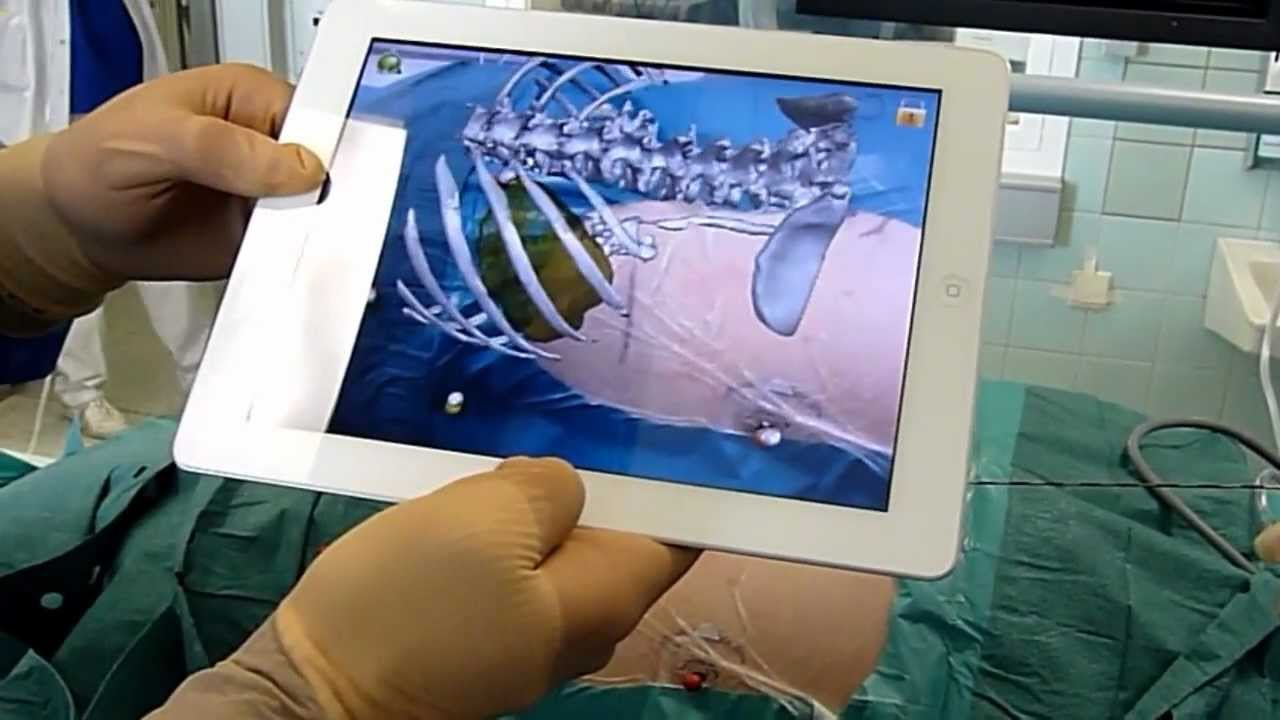
\includegraphics[width=1.00\textwidth]{images/mobile_ar_medical.jpg}
    \caption{Augmented Reality application in Medical field}
    \label{fig:ar_medical}
\end{figure*}

\subsubsection{Medical}
Augmented Reality could be used by Doctors as a visualization and training aid for surgery, as shown in Figure \ref{fig:ar_medical}. A novice surgeon could consult with a highly trained surgeon. Virtual instructions could remind him of the required steps, without the need to look away from the patient or consult a manual and all this could be done remotely without the need of the physical presence of the professional there. In her TED talk \cite{Hachach-Haram2017}, Nadine Hachach-Haram showed how AR is currently revolutionizing the medical industry and how this could potentially benefit those with low infrastructural and educational facilities.


\subsubsection{Manufacturing and Repair}
Another application of Augmented Reality is the assembly, maintenance and repair of complex machinery as the instructions might be easier to understand if, instead of reading manuals, it was available as 3D drawings with step by step instructions as to how to perform some task, as shown in Figure \ref{fig:ar_repair}.

\begin{figure}[H]
    \centering
        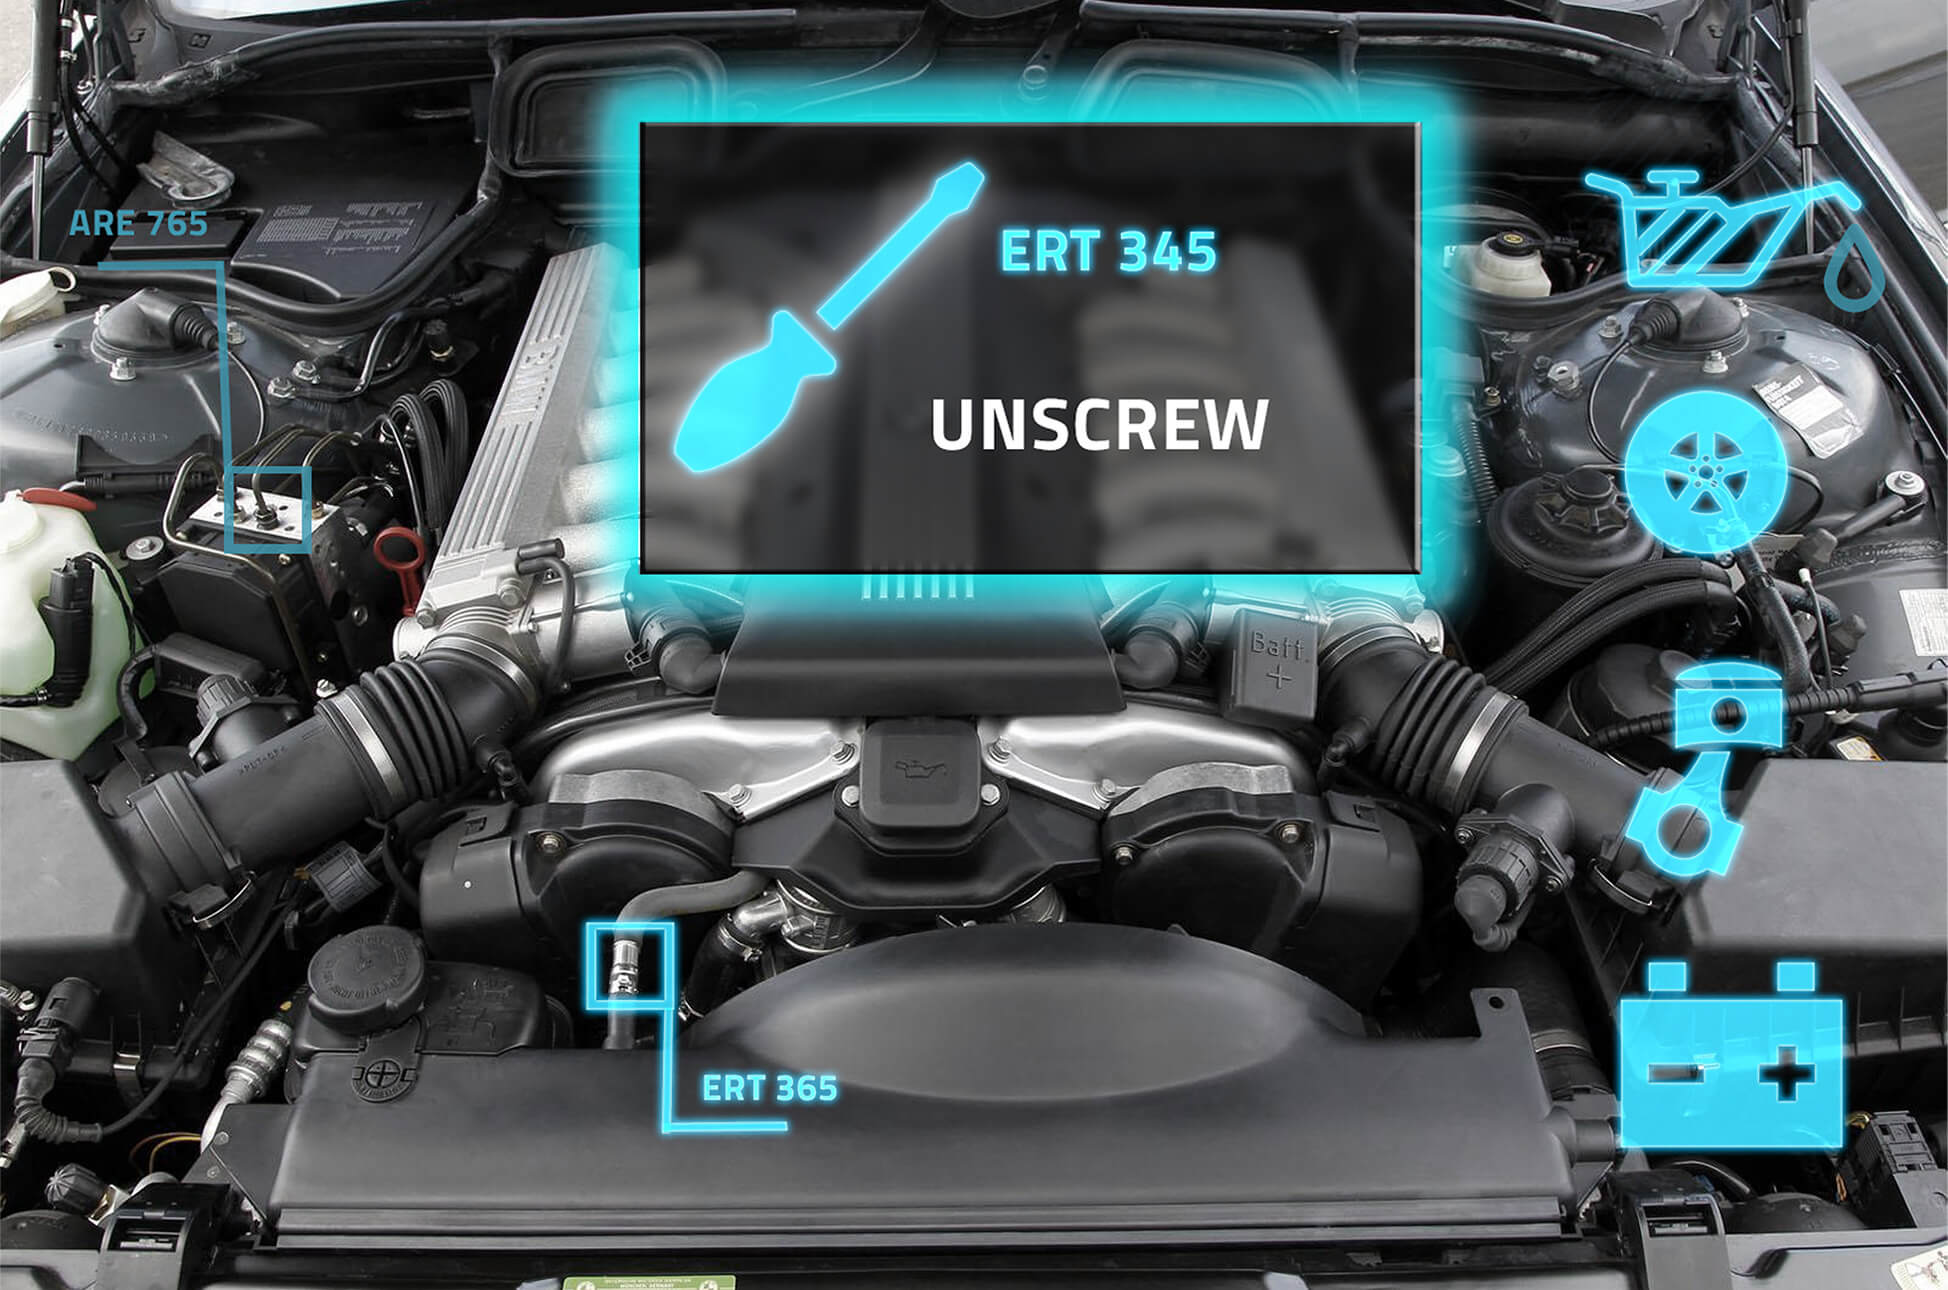
\includegraphics[width=0.90\textwidth]{images/ar_repair.jpg}
    \caption{AR usage in Engine Repairing}
    \label{fig:ar_repair}
\end{figure}


\subsubsection{Annotation and visualization}
AR could also be used for annotations and visualization purposes, where it annotates an object with some relevant information, as shown in Figure \ref{fig:ar_annotation}. For this purpose, it would fetch information from some public database, or it could also be some privately maintained database, as is the case in our application. Our use-case for the current project falls under this category as we are annotating or visualizing the current location of the user in the real-world using Augmented Reality.

\begin{figure}
    \centering
        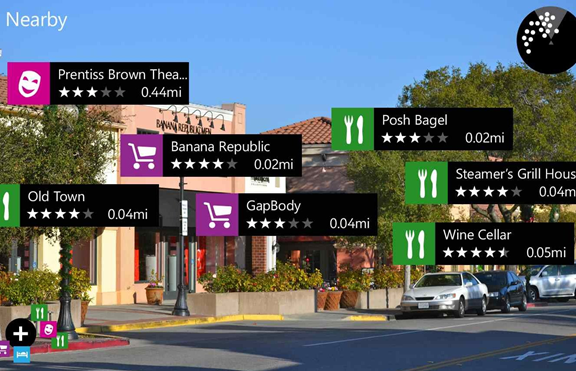
\includegraphics[width=1.00\textwidth]{images/ar_annotation.png}
    \caption{Annotation of Nearby Places in AR}
    \label{fig:ar_annotation}
\end{figure}


\subsubsection{Navigation}
Augmented Reality could also be used for navigation purposes where some markers of lines are superimposed onto the paths that the user needs to follow. Mapbox \cite{MapboxAR2017}, as well as Google \cite{Maps2018}, worked on this problem to make it more efficient and reliable to work on World-scale AR. In Figure \ref{fig:ar_navigation_maps}, Google revealed how their Google Maps apps would use Augmented Reality, both in Android as well as iOS, to help users navigate through the real world \cite{Maps2018}.

\subsubsection{Entertainment}
In the past couple of years, AR has been used extensively in this area, from Facebook and Snapchat Filters to games like Pokemon Go, as shown in Figure \ref{fig:ar_pokemongo}, it has helped a lot in publicity of Augmented Reality technology. With the advent of Mobile AR, numerous apps have been released that make use of this technology to entertain their users.

\begin{figure}
    \centering
        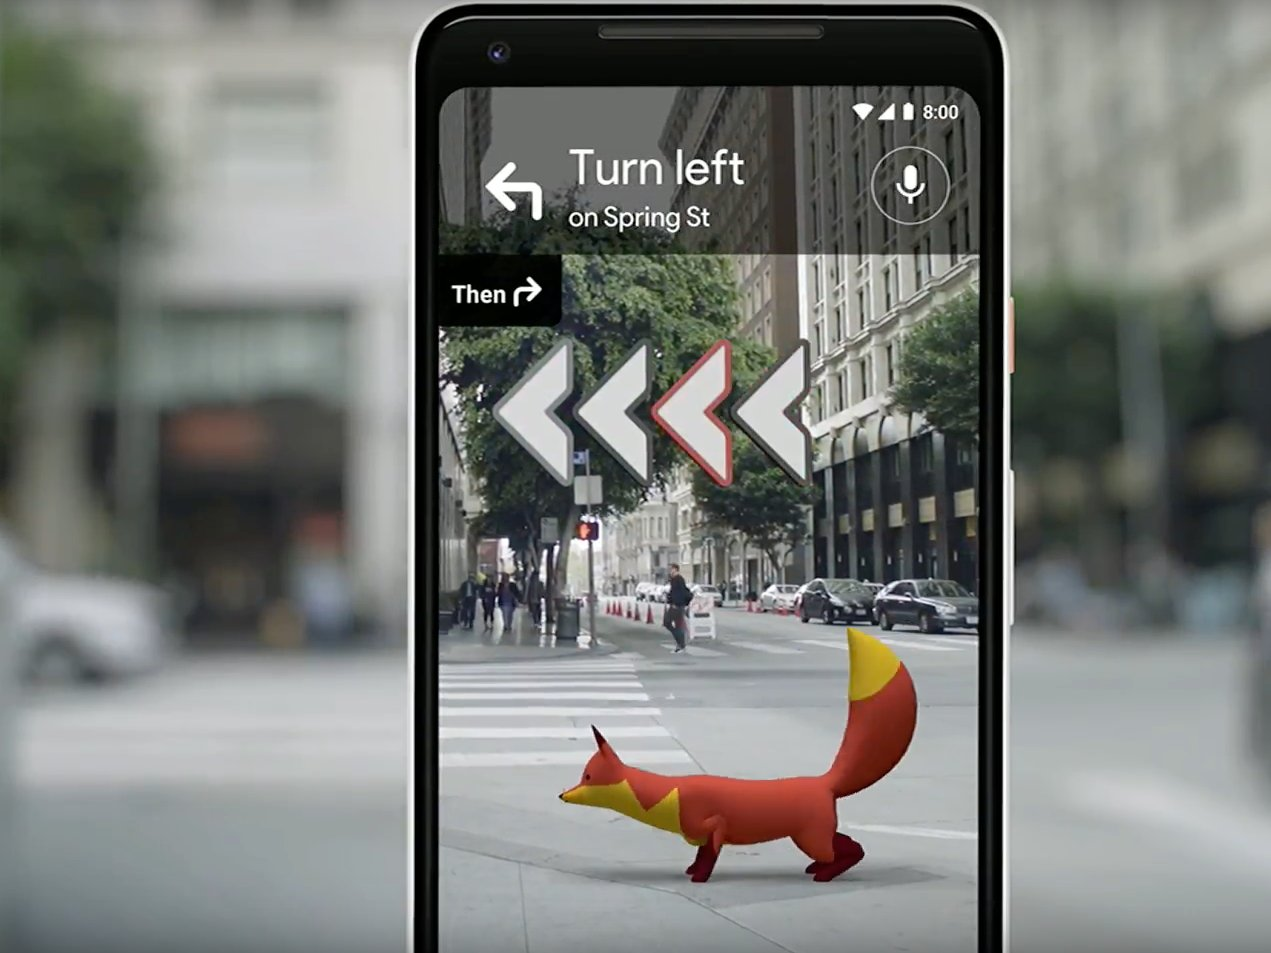
\includegraphics[width=1.00\textwidth]{images/ar_navigation_maps.png}
    \caption{AR Navigation in Google Maps}
    \label{fig:ar_navigation_maps}
\end{figure}




\begin{figure}
    \centering
        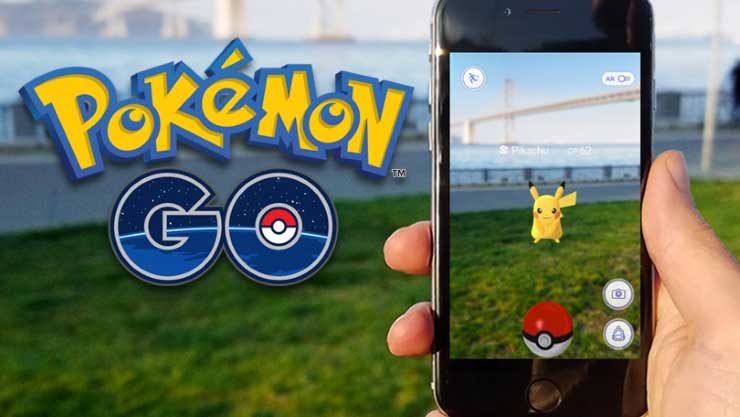
\includegraphics[width=1.00\textwidth]{images/ar_pokemongo.jpg}
    \caption{Use of AR in Pokemon Go}
    \label{fig:ar_pokemongo}
\end{figure}

\subsection{Mobile AR}
There are some specific devices designed for AR usage, but they tend to be pricey and not yet economical and practical. Mobile AR is where AR technology is used on our daily smart-phones, tablets, etc., instead of those specialized AR glasses and hardware \cite{craig2013understanding}. There has been a surge in past couple of years in the usage of Mobile AR because of little to no investment on the part of end-users. Developers have been using it extensively to deliver new and unique experiences to their users, and tech-giants like Apple and Google are battling for the dominance in this area. There are over 2000 AR apps available in iOS Store and another 200-plus on Google Play \cite{Moon2018}.

Apple released their AR library, named ARKit \cite{ARKitDevelopers2018}, which was very well received by the developer's community. It was soon followed by ARCore \cite{ARCoreDevelopers2018}, which was released by Google. Both libraries were focused on solving the same problem, introducing AR on a mobile platform and to dominate this area. As ARKit was released earlier, that is the reason behind a vast number of AR apps on iOS Store as compared to Google Play. Another thing is that ARCore can only run on some specific hardware devices. They have a list of supported devices that they update with time as the library matures and the hardware gets powerful enough to support AR \cite{ARCoreSupportedDevices2018}.

We decided to use ARCore for our project as it was relatively new at that point and the cost of development of Android apps is low as compared to iOS apps. Besides we already had experience building Android apps before, so it was more feasible for us just to use Android for the project and focus on learning to integrate AR into our app instead of learning to program for whole another platform.

\section{Firebase}
Firebase is a mobile and application development platform which was developed by Firebase, Inc but later was acquired by Google\cite{FirebaseWikipedia2018}. 

\subsection{Services}
Firebase offers a range of services to the developers that make app development easier for them. Some of the most popular services include \cite{Firebase2018}:
\begin{description}[font=$\bullet$~, leftmargin=0cm]
    \item[Google Analytics] Analyzes user attributions and behavior and provides a single dashboard for visualizing and managing it.
    \item[Authentication] Provides a simple way to authorize users through multiple methods, including email and password and third-party services like Google, Facebook, etc.
    \item[Cloud Functions] Custom back-end code that gets triggered by some specified events and executes and scales automatically without needing to manage your own servers.
    \item[Realtime Database] Store and sync data between different users and devices in realtime using NoSQL database, updated data syncs in milliseconds regardless of network connectivity.
    \item[Cloud Messaging] Send messages and notifications to users, either single devices or groups of devices, across platforms, Android, iOS, and web, for free.
\end{description}

\subsection{Motivation}
We chose Firebase because of the services it provides and because of the great documentation behind it and how deeply it is integrated into the Android development ecosystem. The main services that we used are \textbf{Authentication} and \textbf{Realtime Database}. We used Realtime Database to update a user's location in real-time and sync it with their contacts. We also used it to introduce real-time chatting into our application.

Another big reason why we chose Firebase is their Free-tier pricing plan \cite{FirebasePricing2018} and automatic plan upgrade if the app needs more resources. One of the primary motivations behind this project was to make it more economical, use as little resources as possible and spend as little money on it as possible. This will result in providing better services to the users free of cost.


\section{Summary}
Our proposed system will track the location of the users in real-time and store it in Firebase which is a remote real-time database. It will use ARCore, which is an AR library for Android platform, for the visualization of a user's location in the real-world. It will also add support for real-time chatting as well as a chat bot, so the users could have an enjoyable and a rewarding experience.



